\documentclass{article} % For LaTeX2e
\usepackage{nips15submit_e,times}
\usepackage{hyperref}
\usepackage{url}
\usepackage{graphicx}
\graphicspath{ {/Users/Tyler/LOVEFest/Figures/pdf/} }
%\documentstyle[nips14submit_09,times,art10]{article} % For LaTeX 2.09
\usepackage{amsfonts,amsmath,amssymb,amsthm}
\usepackage{color}
\usepackage{paralist}

\usepackage{algorithm}
\usepackage{algpseudocode}

\providecommand{\tt}[1]{\textcolor{blue}{\it tt says: #1}}
\newcommand{\jovo}[1]{{\color{magenta}{\it jovo says: #1}}}

\floatname{algorithm}{Procedure}
\renewcommand{\algorithmicrequire}{\textbf{Input:}}
\renewcommand{\algorithmicensure}{\textbf{Output:}}

\newcommand{\Real}{\mathbb{R}}
\providecommand{\mc}[1]{\mathcal{#1}}
\providecommand{\mt}[1]{\widetilde{#1}}
\providecommand{\mh}[1]{\hat{#1}}
\newcommand{\T}{^{\ensuremath{\mathsf{T}}}}           % transpose
\newcommand{\argmax}{\operatornamewithlimits{argmax}}
\newcommand{\argmin}{\operatornamewithlimits{argmin}}


\title{Randomer Forests}


\author{
Tyler M. Tomita\thanks{ Use footnote for providing further information
about author (webpage, alternative address)---\emph{not} for acknowledging
funding agencies.} \\
Department of Biomedical Engineering\\
Johns Hopkins University\\
Baltimore, MD \\
\texttt{ttomita@jhu.edu} \\
\And
Mauro Maggioni \\
Department of Mathematics \\
Duke University \\
Durham, NC \\
\texttt{mauro@math.duke.edu} \\
\And
Joshua T. Vogelstein \\
Department of Biomedical Engineering \\
Johns Hopkins University \\
Baltimore, MD \\
\texttt{jovo@jhu.edu} \\
}

% The \author macro works with any number of authors. There are two commands
% used to separate the names and addresses of multiple authors: \And and \AND.
%
% Using \And between authors leaves it to \LaTeX{} to determine where to break
% the lines. Using \AND forces a linebreak at that point. So, if \LaTeX{}
% puts 3 of 4 authors names on the first line, and the last on the second
% line, try using \AND instead of \And before the third author name.

\newcommand{\fix}{\marginpar{FIX}}
\newcommand{\new}{\marginpar{NEW}}

\nipsfinalcopy % Uncomment for camera-ready version

\begin{document}

\maketitle

\begin{abstract}
\jovo{please make this submittable asap.  this means include bib, put figures in the right place, anonymize, etc.}
\end{abstract}

\section{Introduction}

% \paragraph{Opportunity} 
Data science is becoming increasingly important as our ability of a society to collect and process data continues to increase.  Supervised learning---the act of using predictors to make a prediction about some target data---is of special interest to many applications, ranging from science to government to industry.  Classification, a special case of supervised learning, in which the target data is categorical, is one of the most fundamental learning problems, and has been the subject of much study.  A simple pubmed search for the term ``classifier'' reveals nearly 9,000 publications, and a similar arXiv search reports that the number of hits is $>$1000.  One of the most popular and best performing classifiers is random forests (RFs) \cite{Breiman2001}.  Several recent benchmark papers assess the performance of many different classifiers on many different datasets \cite{Delgado2014,Caruana2008}, and both concluded the same thing: random forests are the best classifier.

The reasons for the popularity and utility of random forests are many. Below, we list some of the reasons, in order of approximate importance (as assessed subjectively and qualitatively by us):
\begin{compactitem}
\item \textbf{empirical performance}: excellent prediction performance in a wide variety of contexts;
\item \textbf{scale and unit invariance}: different predictor variables can have totally different units, e.g. millimeters and kilograms, for example, without affecting RF's;
\item \textbf{robust to outliers}: certain data points could be outliers, either because some or all of the values of their feature vector are far from the others;
\item \textbf{computational efficiency}: it is reasonably efficient, more so than an exhaustive search to find the globally optimal tree, which is NP-hard \cite{Heath1993};
\item \textbf{interpretability}: it is reasonably interpretable, as each variable can be assigned an importance score (such as the ``gini'' score), albeit for large forests it can become hard to sort the variables in order of importance;
\item \textbf{storage efficiency}: when training on lots of data, storage of the classifier can become problematic.
\end{compactitem}


% \paragraph{Challenge}
Although the benefits of RF are many, there is room for improvement. The main drawback of using RFs, in our opinion, is its sensitivity to rotations and other operations that ``mix'' variables.  While RFs usually refers to Breiman's Forest-IC, which uses axis-parallel \cite{Heath1993}, or orthogonal trees \cite{Menze2011}, Breiman also characterized Forest-RC, which used linear combinations of coordinates rather than individual coordinates, to split along.  Others have studied several different variants ``oblique'' random forests, including efforts to learn good projections \cite{Heath1993,Tan2004}, or using principal components analysis to find the directions of maximal variance \cite{Ho1998,Rodriguez2006}, or directly learn good discriminant directions \cite{Menze2011}.  While these approaches deal with rotational invariance, they all also lose at least one of the above benefits of RF, namely scale invariance.  The scale invariance property of RF is one of its most important and special properties, distinguishing it from most other classifiers, and making it appropriate in a wider variety of contexts.  

%Although the benefits of RF are many, as with everything, there is room to improve. The main drawback of using RFs, in our opinion, is its sensitivity to rotations.  Because when people refer to RFs they often mean Breiman's Forest-IC, which uses axis-parallel \cite{Heath1993}, or orthogonal trees \cite{Menze2011}, Breiman also characterized Forest-RC, which used linear combinations of coordinates rather than individual coordinates, to split along.  Others have studied several different variants ``oblique'' random forests, including efforts to learn good projections \cite{Heath1993,Tan2004}, or using principal components analysis to find the directions of maximal variance \cite{Ho1998,Rodriguez2006}, or directly learn good discriminant directions \cite{Menze2011}.  While each of these approaches deal with rotational invariance, they all also lose at least one of the above benefits of RF, namely scale invariance.  The scale invariance property of RF is one of its most important and special properties, distinguishing it from most other classifiers, and making it appropriate in a wider variety of contexts.  

Moreover, all of the above approaches become outlier sensitive, and lose computational and storage efficiency.
There is therefore a gap that calls for the construction of a classifier that has excellent empirical performance, while maintaining scale invariance, as well as robustness and computational and storage efficiency.

% \paragraph{Action}
To bridge this gap, we first state a generalized forest building scheme, linear threshold trees, which includes all of the above algorithms as special cases.  This enables us to formally state our objective, and provides a lens that enables us to propose a few novel special cases, which we refer to as ``{\em{Randomer Forests}}''  (or RerFs for short), for reasons that will become clear in the sequel.  We both theoretically and empirically demonstrate that our methods have the same time and space complexity as random forests, while matching or exceeding their performance even on axis aligned data.  Moreover, we demonstrate that a variant of RerF is approximately is both affine invariant and robust to outliers, two properties that are relatively easy to obtain independently, though difficult to obtain jointly and inexpensively (see recent work on robust PCA following \cite{Candes2009}). Finally, we demonstrate on a suite of benchmark datasets, that RerF outperforms RF in terms of both accuracy and interpretability.  We conclude that RerF should be the new reference classifier.


% \paragraph{Resolution}

% \paragraph{Future}

% Ensemble classification methods have demonstrated much success in recent years (cite). One reason ensembles work well is because averaging the votes of many weak classifiers can substantially reduce the variance. Another reason is that the ensemble may provide a better approximation to the true function $f$ when the hypothesis space of individual classifiers does not contain a good approximation (Dietterich 2002). Two factors that have a significant impact in the performance of an ensemble method are \textit{diversity} and \textit{accuracy} (Margineantu and Dietterich 1997). Accuracy describes the ability of each individual classifier to generalize to new points, while diversity quantifies the amount of correlation between generalization errors of individual classifiers. It is easy to see that if all individual classifiers are completely accurate, then no benefit is gained using an ensemble. However, if individual classifiers are weak but diverse, the ensemble can have marked improvement in performance over any of the individual ones.

% One ensemble method in particular that has been shown to work well in a variety of settings is random forests (Breiman 2001). Recent studies evaluating many different classifiers on a wide range of datasets have shown random forest classifiers to exhibit the overall best performance across all classifiers examined (Caruana;Delgado). A random forest is a diverse ensemble of decision trees, where diversity is introduced through a combination of bagging (cite) and random subsampling of predictors at each split node of each tree. While random forests has demonstrated marked success, decision boundaries associated with each split node are restricted to alignment with the coordinate axes. We believe that such a restriction limits both the accuracy as well as the diversity of the resulting ensemble classifier. In this paper, we propose a new method, called randomer forests, which removes the restriction of axis-aligned partitions. The main heuristic is in replacing random subsampling of predictors in random forests with sparse random projections. 

% \jovo{outlines of the paper are verbose, and it should be clear from the introductory content what you will be doing. i removed yours}

% Details of the implementation of our method are described in section 2. In section 3, we evaluate the performance of our method on both simulated and real datasets. Furthermore, we explore robustness of our method against various transformations and outliers.

\section{Linear Threshold Forests}

A classification forest, $\bar{g}_n(X; \mc{D}_n)$ is an ensemble of decision trees, each of which is trained on a (sub)set of the data, $\mc{D}_n=(X_i,y_i)$ for all $i \in [n]$, and $X \in \Real^{p \times n}$. Linear threshold forests are a special case of classification forests that subsume all of the strategies mentioned above (see Pseudocode \ref{pseudo}).  The key idea of all of them is that at each node, given $\bar{X} \in \Real^{p \times s}$---the set of predictors in the node---we sample a  matrix $A \sim f_A(\mc{D}_n)$, where $A \in \Real^{p \times d}$ possibly in a data dependent fashion, which we use to project the predictor matrix $X$ onto a lower dimensional subspace, yielding $\mt{X} = A\T X \in \Real^{d \times s}$, where $d \leq p$ is the dimensionality of the subspace, and $s \leq n$ is the number of samples at the given node.  To wit, Breiman's original Forest-IC algorithm can be characterized as a special case of linear threshold forests.  In particular, in Forest-IC one constructs $A$ such that for each of the $d$ columns, we sample a coordinate (without replacement), and put a 1 in that coordinate, and zeros elsewhere. Similarly, Ho's rotation forests construct $A$ from the top $d$ principal components of the data $\bar{X}$ at a given node.  Thus, the key difference in all these approaches is the choice of $f_A$. 


\begin{algorithm}
\caption{Psuedocode for Linear Threshold Forests, which generalizes a wide range of previously proposed decision forests.} \label{pseudo}
\begin{algorithmic}[1]
\Require 
% \begin{compactitem}
\State {Data}: $\mc{D}_n = (X_i,y_i) \in (\Real^p \times \mc{Y})$ for $i \in [n]$
\State {Tree rules}:  $n_{tree}$, stopping criteria, pruning rules, rule for sampling data points per tree, etc.
% \State \textbf{distribution on $[n]$}: $\mc{S}^l \sim f_s$ , where $\mc{S}^l \subset [n]$  is the index set of data points for tree $l$ 
% \item \textbf{Subspace}: $\mc{A}^{p \times d}$
\State {Distributions on $s \times d$ matrices}: $A \sim f_A(\mc{D}_n)$, for all $s \in [n]$
% \item \textbf{Stoppping criteria}: e.g., a maximal tree depth or minimum number of elements per tree 
% \end{compactitem}
\State Preprocessing rules
\Ensure decision trees, predictions, out of bag errors, etc. 
\State Preprocess according to rule
\For{each tree}
\State Subsample data to obtain $(\bar{X},\bar{y})$, the set of data points to be used in this tree
\For{each leaf node in tree}
\State Let $\mt{X} =  A\T \bar{X} \in \Real^{d \times s}$, where $A \sim f_A(\mc{D}_n)$
\State Find the coordinate $k^*$ in $\mt{X}$ with the ``best'' split
\State Split $X$ according to whether $X(k) > t^*(k^*)$
\State Assign each child node as a leaf or terminal  node according to convergence criteria
\EndFor
\EndFor
\State Prune trees according to rule
\end{algorithmic}
\end{algorithm}

The goal of this work is to find a linear threshold forest that has all of the desirable properties of random forests, as well as being approximately affine invariant, in part by changing the distribution $f_A$. The result we call randomer forests (or RerFs for short).


\section{Randomer Forests}

Our construction has $3$ key ingredients, each one designed to address one of the benefits/drawbacks of random forest.
First, we address the {\em{rotation sensitivity}}.  It is well known that principal components are rotationally invariant, but can be expensive to compute and are biased towards directions of large variance vs. directions that may be useful for classification. Instead we use random projections: we generate matrices $A$ that are distributed in a rotation invariant fashion, but maintain the space and time complexity of RFs, by employing very {\bf{sparse random projections}} \cite{Li2006}.  Rather than sampling $d$ non-zero elements of $A$, enforcing that each column gets a single non-zero number (without replacement), which is always $1$, we relax these constraints and select $d$ non-zero numbers from $\{-1,+1\}$ with equal probabilities and distribute uniformly at random in $A$. The result is equally sparse as RFs, but nearly rotationally invariant.  Note that this aspect of RerFs is quite similar to Breiman's Forest-RC, although he used entries in the interval $[-1,1]$, amongst other minor differences. Denote linear threshold forests that use the above scheme for sampling $A$ matrices RerFs.  Figure \ref{fig:cigars}(A) and (D) depicts the difficulty of RF performing in even a very simple scenario, versus RerF \ref{fig:cigars}(B), which does exceptionally well.


\begin{figure}[h]
\begin{center}
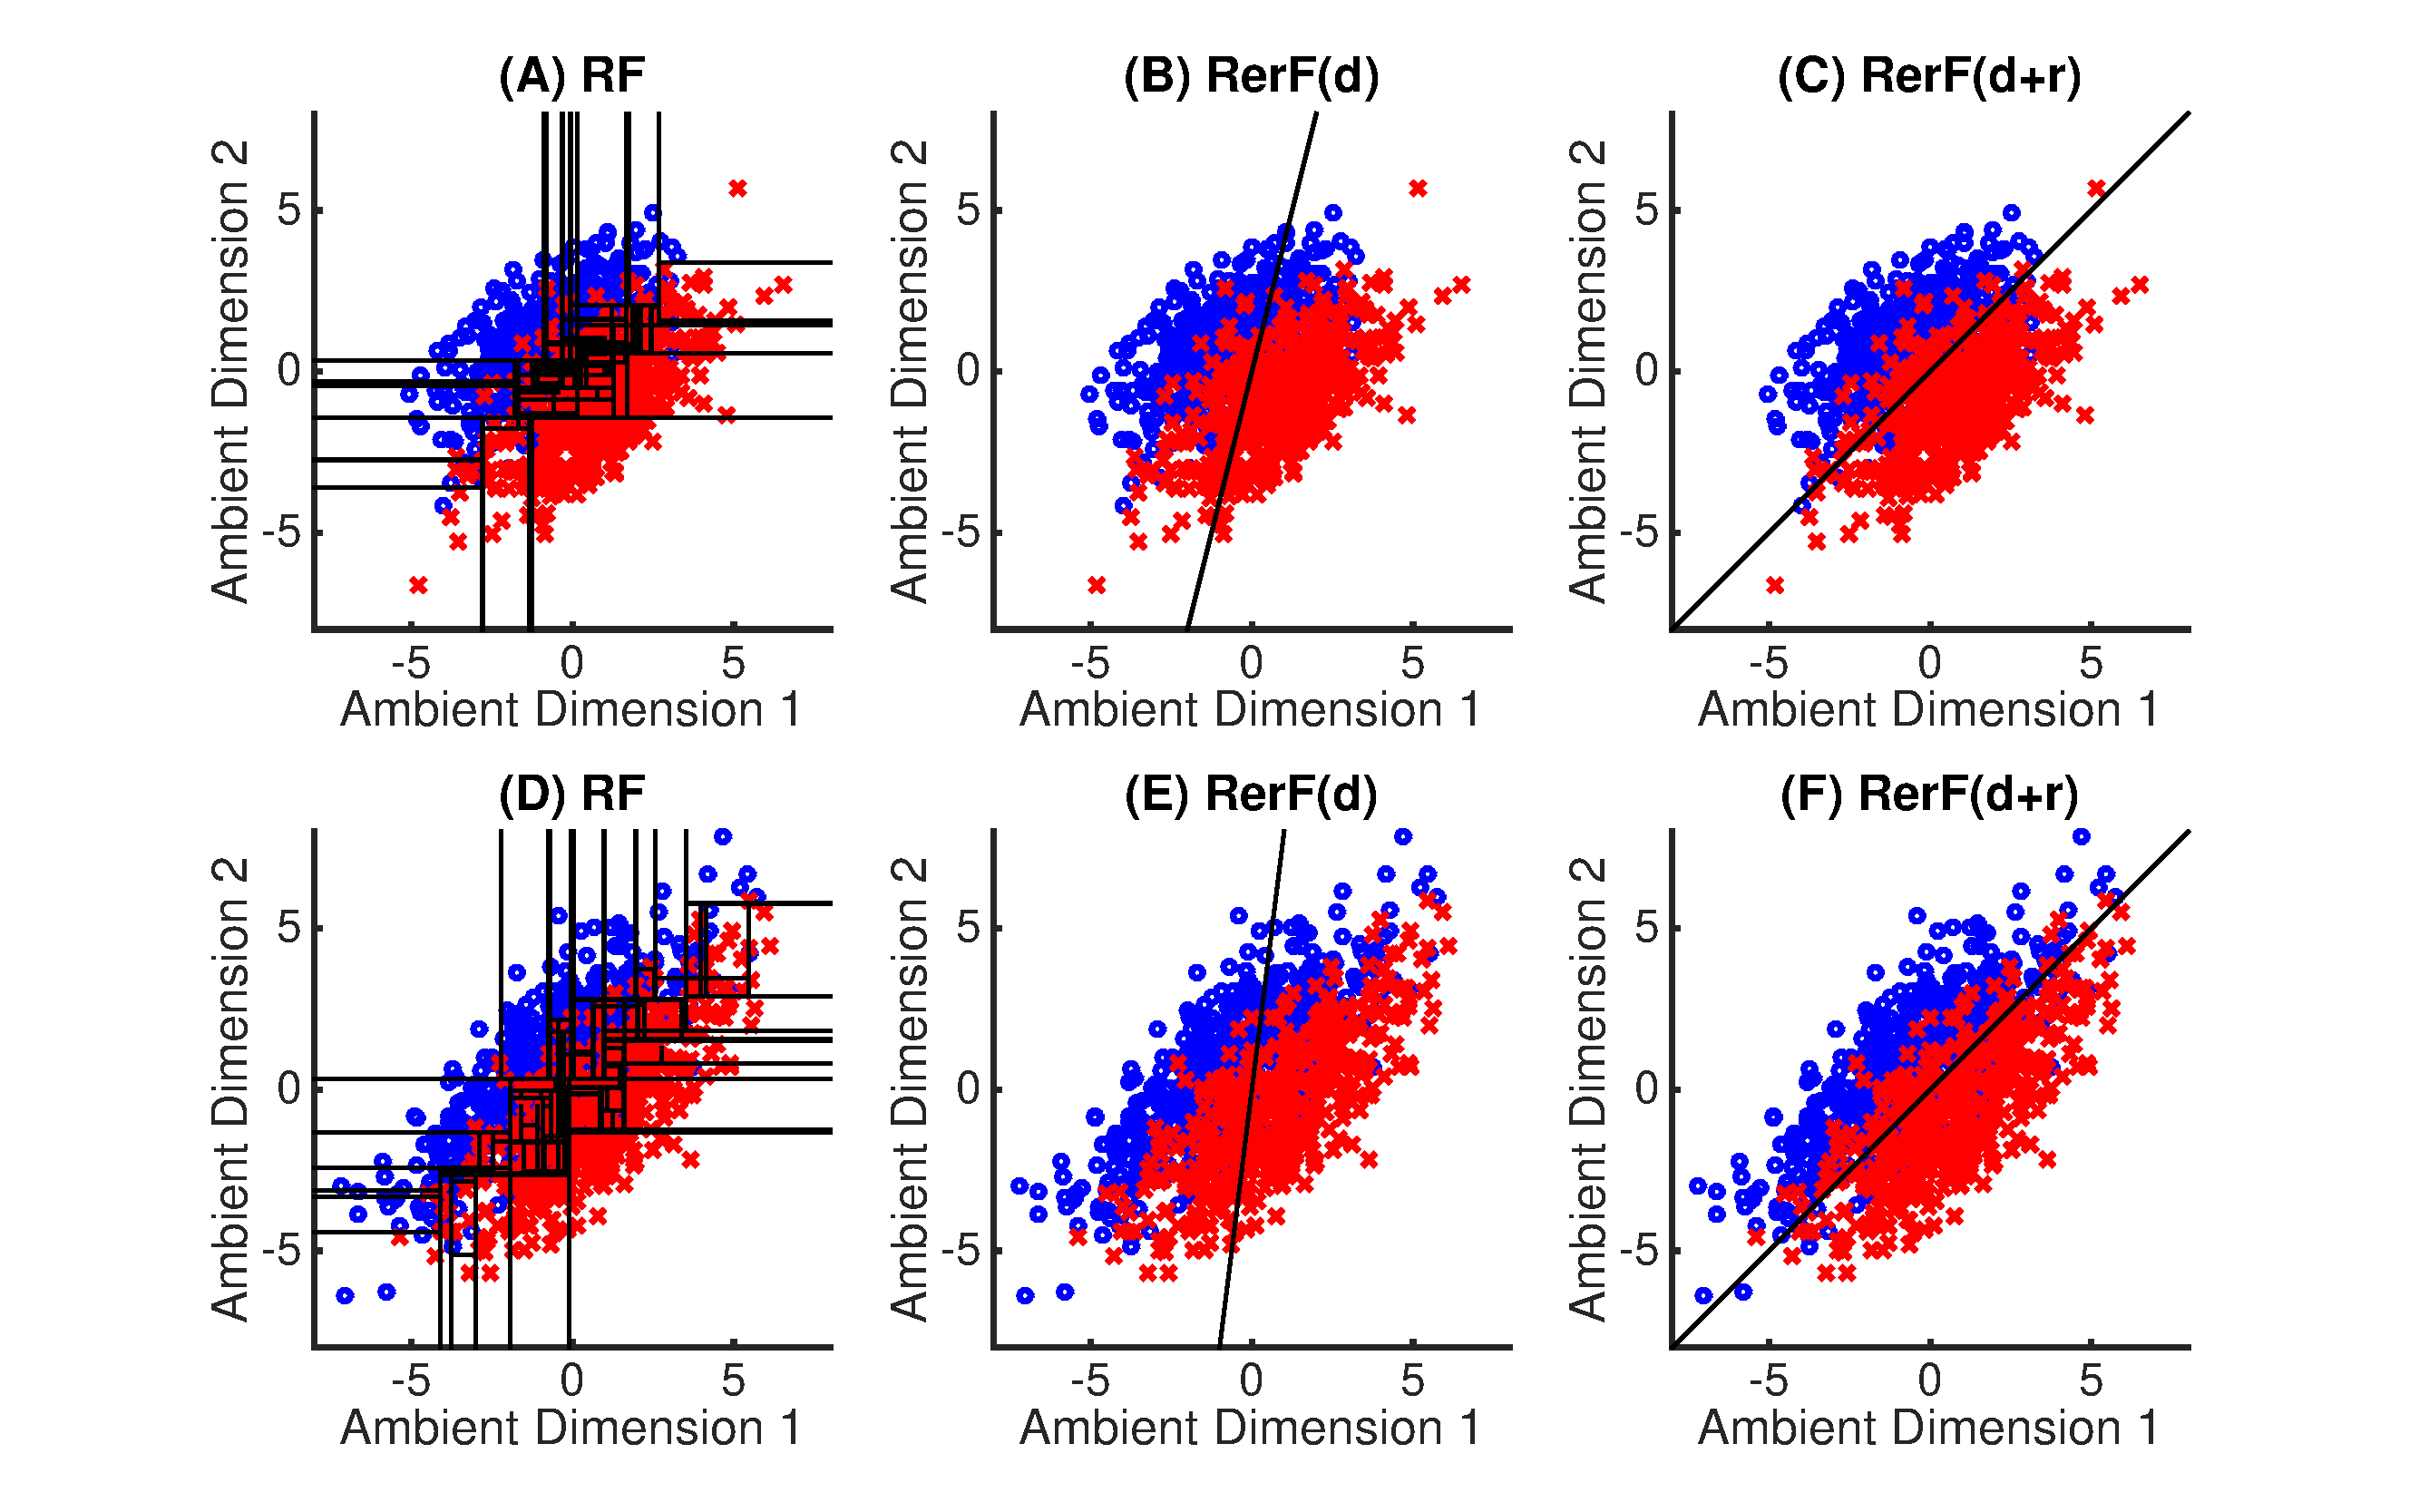
\includegraphics[trim=0in 3.2in 0in 3in, clip=true, width=\linewidth]{../Figures/pdf/Cigars}
\end{center}
\caption{Scatter plot of parallel cigars in two dimensions. 1000 samples are obtained from multivariate Gaussians, where $\mu_j=[j, 0]$, for $j \in \{-1,1\}$, and $\Sigma$ is a diagonal matrix with diagonal elements $(1,8)$.  The data are then rotated by 45 degrees. (A) Decision boundaries from a single tree of RF. (B) The decision boundary obtained by projecting the input data onto the difference in class-conditional means. (C) The same as (B), but first passing the input to ranks before computing the difference in means.}
\label{fig:cigars}
\end{figure}

Unfortunately, by mixing dimensions of $X$, we lost {\em{scale and unit invariance}}.  In fact, all previously proposed oblique random forests, that we are aware of, have lost scale and unit invariance.  We therefore note that random forests have a special property: they are invariant to monotonic transformations of the data applied to each coordinate in the ambient (observed) space.  They are effectively operating on the order statistics, rather than actual magnitudes of coordinates.  In other words, if we convert, for each dimension, the values of the samples to their corresponding ranks, random forests yield the exact same result. Therefore, for our second trick, we adopt the same policy, and ``{\bf{pass to ranks}}'' prior to doing anything else. Denote RerFs that pass to ranks RerF(r).
Figure \ref{fig:cigars}(E) demonstrates that RerF does not work well when the different dimensions are scaled quite differently from one another, but RerF(r) rectifies the situation, and does no harm in the other case. 

Finally, the above two tricks do not {\em{use the data to construct $A$ at each node}}.  Yet, there is  evidence that doing so can significantly improve performance \cite{Heath1993}.  However, previously proposed approaches use methods that are time- and space-intensive compared to standard random forests.  We propose a simple strategy: compute the mean difference vector.  In other words, given a two-class problem, let $\mh{\delta}=\mh{\mu}_0-\mh{\mu}_1$, where $\mh{\mu}_c$ is the estimated class conditional mean.  Under a spherically symmetric class conditional distribution assumption, $\mh{\delta}$ is the optimal projection vector.  When there are $C>2$ classes, the set of all pairwise distances between $\mh{\mu}_c$ and $\mh{\mu}_{c'}$ is of rank $C-1$.  Because RerFs are approximately rotationally invariant, we can simply compute all the class conditional means, and subtract each from one of them (we chose the $\mh{\mu}_c$ for which $n_c$, the number of samples in that class, is the largest). {\bf{MM:say how these differences are used in the thresholding step....}}
Computing this matrix is extremely fast, because it does not rely on costly singular value decompositions, matrix inversions, or convex problems.  Thus, it nicely balances using the data to find good vectors, but not using much computational space or time. Denote RerFs that include this matrix RerF(d), and if they pass to ranks first, RerF(r+d).

%\subsection{Simulated Data}
%We constructed three synthetic datasets (Trunk, parity, and multimodal) to compare classification performance (Fig \ref{fig:1}) and training time (Fig \ref{fig:2}) of RerF, RerF($\delta$), and RerF($\delta$+r) with that of random forest. Trunk is a well-known binary classification \cite{Trunk1979} in which each class is distributed as a p-dimensional multivariate gaussian with identity covariance matrices. The means of the two classes are $\mu_1 = (1,\frac{1}{\sqrt{2}},\frac{1}{\sqrt{3}},...,\frac{1}{\sqrt{p}})$ and $\mu_2 = (-1,-\frac{1}{\sqrt{2}},-\frac{1}{\sqrt{3}},...,-\frac{1}{\sqrt{p}})$. Parity is a binary classification problem in which each of the two classes is distributed as a mixture of $2^{p-1}$ multivariate gaussians with covariance matrices $\boldsymbol{\Sigma} = \frac{1}{32}\boldsymbol{I}$. The means of class one are the subset of $[0,1]^p$ for which the number of zeros in a mean is even. The means of class two are the subset of $[0,1]^p$ for which the number of zeros in a mean is odd. Multimodal is a four-class classification problem. Each of the four classes is distributed as an equal mixture of two multivariate gaussians. The means are randomly sampled from a p-dimensional multivariate standard gaussian and the covariance matrices are sampled from an inverse Wishart distribution with $10p$ degrees of freedom and  a mean covariance matrix equal to the identity matrix. The bottom panels of Figure 1 depict scatter plots of the data for $p=2$. The top panels depict average misclassification rate over ten trials estimated using the out of bag error. For the trunk and multimodal simulations, 100 points were sampled and p varied from two to 1000 dimensions. For the parity simulation, 100 points were sampled and p varied from two to ten. The appropriate number of trees trained for RF and all variants of RerF for trunk, parity, and multimodal were empirically determined to be 1500, 1000, and 500 respectively (Fig \ref{fig:A1}). Bayes error is also included for reference. In binary classification problems in which each class consists of a single multivariate gaussian with equal covariance matrices, such as the Trunk simulation, Bayes error can be computed analytically \cite{Bickel2004}. In the Parity and Multimodal simulations, Bayes error was estimated by averaging the misclassification rate of the Bayes optimal classifier on 1000 points over ten trials.


% A random forest is an ensemble of randomized decision trees, where each decision tree consists of internal (split) and terminal (leaf) nodes. At each internal node, a random subset of the ambient (coordinate) dimensions is sampled and subsequent optimization of a split function selects the single best dimension and split point contained in this subset. Therefore, each tree within a random forest can be viewed as a hierarchical series of axis-aligned decision boundaries. Here, we introduce a new method for constructing randomized decision trees, where instead of random subsampling the dimensions, we randomly project to a lower dimensional subspace. By randomly projecting, decision boundaries are not restricted to alignment with the coordinate axes. Specifically, let $X_i \in \mathbb{R}^{n\times p}$ be a set of $n$ points in $p$ dimensional Euclidean space associated with the ith split node of a decision tree, and let $R_i \in \mathbb{R}^{p\times k}$ be a randomly chosen projection matrix at the ith node. Then for every split node, we compute the projection $X_{proj} = X_iR_i$ and select the optimal split dimension and split point in this randomly chosen k-dimensional subspace.

% There exists various choices for the random projection matrix $R$. If one cares about preserving pairwise distances between points, then $R$ must be chosen carefully. A variety of methods have been established recently for generating random projection matrices that preserve distances. The most common one is to sample each element $r_{ij}$ from a standard normal (Indyk and Motwani, 1998; Dasgupta and Gupta, 2003). Another method generates sparse matrices by setting each element equal to +1 or -1 with probability $1/2\sqrt(p)$ and 0 with probability $1 - 1/\sqrt(p)$ (Li 2006). In this work, we are not concerned with preserving pairwise distances. Rather, we are simply concerned with constructing features at each split node of a tree using linear combinations of the ambient dimensions. We construct random matrices by first, sampling the indices of the k nonzero elements uniformly at random. Next, each nonzero element is randomly assigned -1 or +1 with equal probability. Columns containing all zeros are removed. This results in a matrix with many columns having one nonzero element and a few columns having more than one nonzero element.


% In addition to random projections, for classification problems involving $c$ classes we can compute a set of $c-1$ differences in class-conditional means $\{\boldsymbol{\delta_{ij}} = \boldsymbol{\mu_j} - \boldsymbol{\mu_i}: \forall i \in [1,...,c-1], j \in [2,...,c], j>i\}$ and sample each of them as a projection with probability $k/p$. Such supervised projections work especially well when all classes are normally distributed with diagonal covariance matrices, and are often useful even when these conditions are not met. We denote RerFs utilizing these projections as RerF(d)

% When taking linear combinations of ambient dimensions, it is important that the dimensions be scaled similarly. Therefore we also formulate a variant of RerF in which input data is passed to marginal ranks prior to training. Doing so not only scales the dimensions appropriately, but also can improve performance when outliers are present. This robust variant of randomer forest will be denoted as RerF(r).

\section{Experimental Evaluation}

\subsection{Axis Aligned Simulations}

We constructed three synthetic datasets to compare classification performance (Figure \ref{fig:sim}) and training time (Figure \ref{fig:time}) of RerF, RerF(d), and RerF(r+d) with that of random forest:
% \begin{compactenum}

\textbf{Trunk} is a well-known binary classification in which each class is distributed as a p-dimensional multivariate Gaussian with identity covariance matrices \cite{Trunk1979}. The means of the two classes are $\mu_1 = (1,\frac{1}{\sqrt{2}},\frac{1}{\sqrt{3}},...,\frac{1}{\sqrt{p}})$ and $\mu_2 = -\mu_1$. This is perhaps the simplest axis aligned problem, for which random forests should perform exceedingly well.  

\textbf{Parity} is one of the hardest two-class classification problems, it is a multivariate generalization of the XOR problem.  A given sample has a mean whose elements are Bernoulli samples with probability 1/2, and then Gaussian noise is independently added to each dimension with the same variance.  A sample's class label is equal to the parity of its mean.  This is perhaps the hardest axis aligned problem, for which random forests should do well, whereas linear classifiers will perform at chance.

\textbf{Multimodal} is a four-class classification problem. Each of the four classes is distributed as an equal mixture of two multivariate Gaussians. The means are randomly sampled from a p-dimensional multivariate standard Gaussian and the covariance matrices are sampled from an inverse Wishart distribution with $10p$ degrees of freedom and  a mean covariance matrix equal to the identity matrix.
% \end{compactenum} 

For all comparisons, we used the same number of trees for each method, and the same number of non-zeros when generating $A$, to enable a fair comparison.   The top panels of Figure \ref{fig:sim} shows two-dimensional scatter plots from each of the three example simulations (using the first two dimensions). The bottom panels show the misclassification rate of RF vs RerF and its variants, as well as the Bayes optimal error, against the number of observed dimensions $p$.  In all three cases, RerF(r+d) performs as well or better than RF, even though for the first two, the discriminant boundary is axis aligned.  The reason that RerF outperforms RF even in the axis aligned discriminant boundary cases is that linear combinations of the ambient coordinates can yield new dimensions that have a higher signal to noise ratio than any of the original dimensions.  Therefore, RerF can capitalize on that, and use those dimensions to obtain cleaner splits, and therefore better trees.

% The bottom panels of Figure 1 depict scatter plots of the data for $p=2$. The top panels depict average misclassification rate over ten trials estimated using the out of bag error. For the trunk and multimodal simulations, 100 points were sampled and p varied from two to 1000 dimensions. For the parity simulation, 100 points were sampled and p varied from two to ten. The appropriate number of trees trained for RF and all variants of RerF for trunk, parity, and multimodal were empirically determined to be 1500, 1000, and 500 respectively (Fig A1). Bayes error is also included for reference. In binary classification problems in which each class consists of a single multivariate gaussian with equal covariance matrices, such as the Trunk simulation, Bayes error can be computed analytically (Bickel and Levina 2004). In the Parity and Multimodal simulations, Bayes error was estimated by averaging the misclassification rate of the Bayes optimal classifier on 1000 points over ten trials.


\begin{figure}[h]
\begin{center}
%\framebox[4.0in]{$\;$}
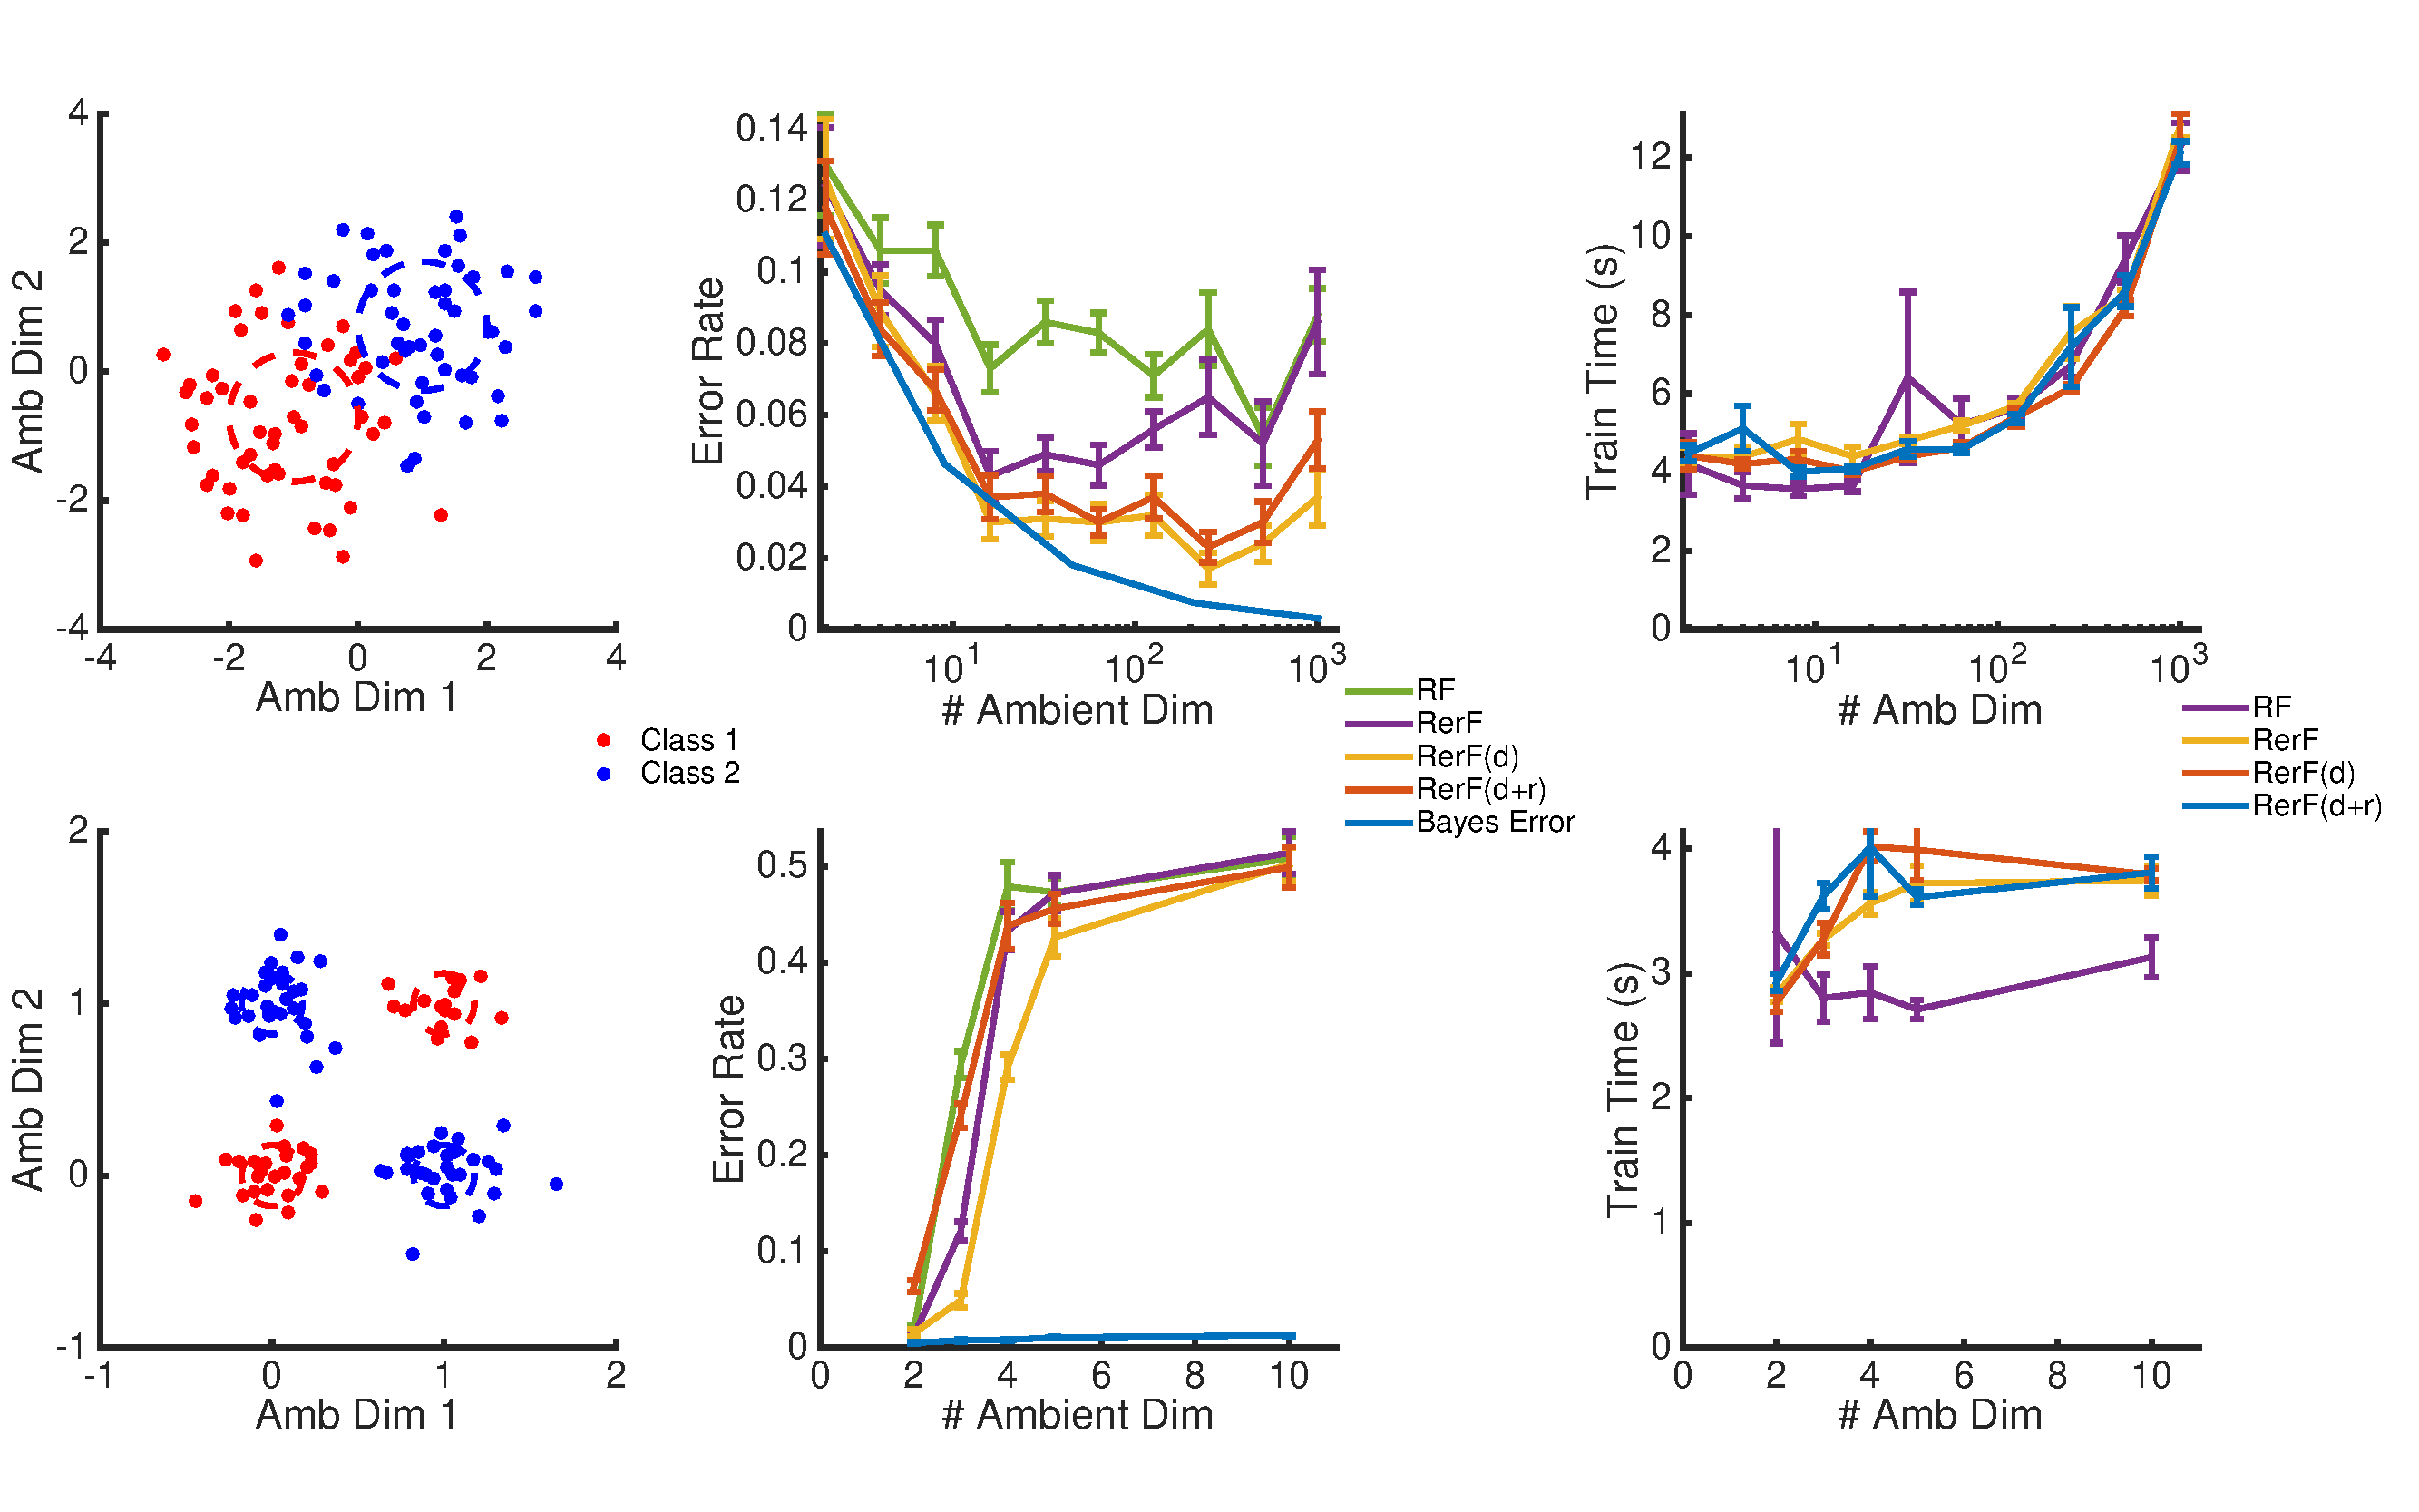
\includegraphics[trim=0in 0in 0in 0in, clip=true, width=\linewidth]{../Figures/pdf/Fig1_Simulation}
\end{center}
\caption{Classification performance comparing Random Forest (RF) to several variants of Randomer Forest (RerF), and Bayes optimal performance, on three distinct simulation settings: (A) Trunk, (B) Parity, and (C) Multimodal (see Methods for details).  For all settings, the top panel shows a 2D scatter plot of the first 2 coordinates (dashed circles denote the standard deviation level set), the middle panel depicts misclassification rate vs. the number of ambient (coordinate) dimensions, and the bottom panel depicts training time comparing RF to several variants of RerF.  Note that in all settings, for all number of dimensions, RerF outperforms RF, even for Trunk and Parity, which were designed specifically for RF because the discriminant boundary naturally lies along the coordinate basis. Although RerF requires slightly more time than RF (largely due to random sampling of projection matrices), they scale similarly. In each case, $n=100$ and the errorbars denote standard error over ten trials.}
\label{fig:sim}
\end{figure}

% Panel A of Figure 1 shows that RerF(d) and RerF(d+r) outperform RF across all numbers of dimensions. This can be attributed to projection onto the difference in means. All variants outperform RF up to approximately 250 dimensions. Above this, misclassification rate of RerF is comparable to RF. In Panel B, we observe that all variants of RerF outperform RF for all numbers of dimensions. This can be understood by observing that for p dimensions, all splits in RF up to a tree depth of $p - 1$ will result in daughter nodes having chance posterior probabilities of being in either class. Therefore, any splits up to this depth that are not aligned with the coordinate axes can only be better. Multimodal???


%Figure \ref{fig:time} shows the corresponding running time for RF and the different RerF variants.  Note that the RerF variants do not take significantly longer to train than RF.  
% , we observe a slight increase training time of all RerF variants compared to RF. Despite this increase, training time for all classifiers scales similarly with the number of dimensions. The apparent increase in training time for the RerF variants is largely due to sampling of the random projection matrices. 


The middle panel of Figure \ref{fig:sim} column A shows that RerF($\delta$) and RerF($\delta$+r) outperform RF across all numbers of dimensions in the Trunk problem. This can be attributed to projection onto the difference in means. All variants outperform RF up to approximately 250 dimensions. Above this, misclassification rate of RerF is comparable to RF. In the middle panel of column B, we observe that all variants of RerF outperform RF for all numbers of dimensions in the parity problem. This can be understood by observing that for p dimensions, all splits in RF up to a tree depth of $p - 1$ will result in daughter nodes having chance posterior probabilities of being in either class. Therefore, any splits up to this depth that are not aligned with the coordinate axes can only be better. Looking at the bottom panels, we observe a slight increase training time of all RerF variants compared to RF in both simulation settings. Despite this increase, training time for all classifiers scales similarly with the number of dimensions. The apparent increase in training time for the RerF variants is largely due to sampling of the random projection matrices. 

\subsection{Theoretical Space and Time Complexity}

For a random forest, assume there are $L$ trees.  
If there are $n$ data points per tree, and each tree grows until terminal nodes have only $\mc O(1)$ data points with $d$ coordinates in them, there are $\mc O(n)$ nodes.
Then the complexity of constructing the random forest, disregarding cross-validation or other randomization techniques for preventing overfitting, is $\mc O(Ln^2d\log n)$. In practice the trees are shallower and stop much earlier than when nodes have $\mc O(1)$ points, so ``in practice'' the complexity often appears to be $\mc O(Lnd\log n)$.
%For each node $k$, it takes $\mc{O}(d)$ time to sample $d$ non-zero numbers per node, and $\mc{O}(d n_k)$ time to subsample the matrix to include only the $d$ features of interest for each of the $n_k$ samples in the node.
%It then takes $\mc{O}(d \log d)$ time to sort to find the best dimension to split on per node.
%Although each node has a different number of samples, the cost at the root node dominates in the best case scenario of well-balanced trees, so we can ignore all the others (up to $\mc O(\log n)$ factors).
%Thus, in total, RF requires $\mc{O}(Ld  (1 + s d\log d))$ time to train. To store the resulting RF, we simply require $\mc{O}(L \log(s))$ space because each node can be represented merely by the index of the coordinate that is used for splitting, plus its threshold.

Randomer forest has a very similar time and space complexity, unlike many of the other oblique random forest variants.  Specifically, assume that RerF also has $L$ trees, and $\mc O(n)$ data points per tree, and no pruning, so $\mc O(n)$ nodes. Like RF, it requires $\mc{O}(d)$ time to sample $d$ non-zero numbers, and $\mc{O}(dn_k)$ time to obtain the new matrix, $\mt{X}$, because it is a sparse matrix multiplication, in node $k$ with $\mc O(n_k)$ nodes.  RerF also takes another $\mc{O}(d/n\log(d/n))=\mc O(1)$ time to find the best dimension. Thus, in total, in the case of well-balanced trees, RerF also requires only $\mc{O}(Ldn^2\log n)$ time to train.  To store the resulting RerF also requires $\mc{O}(L n\log n )$, because each node can be represented by the indices of the coordinates that received a non-zero element, and the expected number of such indices is $\mc O(1)$.  The only additional space constraint is storing which indices are positive, and which are negative, which is merely another constant.
The cost of initially sorting in RerF(r), and of computing the means of the classes in RerF(d) are negligible compared to the main cost above. Note that these numbers are in stark contrast to other oblique random forests.  For example, rotation forests require running a singular value decomposition at each node.


\subsection{Effects of Transformations and Outliers on Classifier Performance}

Given that RerF do as well in misclassification rate as RF in multiple disparate examples, and have time and space complexity comparable, we next want to assess whether we have obtained the desired rotational invariance, while preserving these other properties.  To do so, we consider several different modifications to the above described simulation settings: rotation, scale, affine, and outliers.  To rotate the data, we simply generate rotation matrices uniformly and apply them to the data.  To scale, we applied a scaling factor sampled from a uniform distribution on the interval [0,10]. 
Affine transformations were performed by applying a combination of rotations and scalings as just described. Additionally, we examined the effects of introducing outliers. Outliers were introduced by sampling points from the distributions as previously described but instead using covariance matrices scaled by a factor of four. Empirically, an addition of 20 points from these outlier models to the original 100 points was found to produce a noticeable but not overwhelming effect on classifier performance. For a baseline, we compare RF with RerF variants and Fisherfaces \cite{Fisherfaces}. The misclassification rate for Fisherfaces was estimated using leave-one-out cross validation.

Figure \ref{fig:invar} shows the effect of these transformations and outliers on the Trunk (top) and Parity (bottom) rows. Figure \ref{fig:invar}(A) shows that RF is sensitive to rotations, and therefore affine transformations, but robust to outliers.  Figure \ref{fig:invar}(B) shows that RerF(d) is sensitive to scale, and therefore affine transformations, but not outliers.   Figure \ref{fig:invar}(C) shows that RerF(d+r) is robust to affine transformations and outliers, as desired.  Fisherfaces, which is essentially designed for this example, suffers from scale and therefore affine transformations, as well as outliers.  The Parity example yields a similar result, except that rotating the data helps all the RF and RerF variants.  This is because even $p-1$ dimensional marginal distributions of the data in the ambient coordinates have no class conditional signal.  Thus, rototating the data creates dimensions that have non-zero class conditional signal, which all of the RF and RerF variants can utilize.  On the other hand, Fisherfaces, which is a fundamentally linear classifier, achieves chance levels no matter what.  

%RF does especially well in classification problems in which the optimal decision boundaries are aligned or nearly aligned with the coordinate axes. Rotations in such situations can lead to a decrease in classification performance. Naturally, we wanted to examine the effects of various transformations on classification performance of RerF. These effects were examined using the Trunk and parity simulations as previously described. The transformations we applied were random rotations, scaling, and general affine transformations. Uniformly random rotation matrices were generated by first performing SVD on a p-dimensional matrix in which each element is sampled from a multivariate standard normal distribution. The rotation matrix was taken as the right singular vectors of this SVD. If the determinant of this matrix was equal to $-1$, the first two columns were permuted to render the determinant equal to $+1$. Random scaling was performed by applying to each dimension a scaling factor sampled from a uniform distribution on the interval [0,10]. Affine transformations were performed by applying a combination of rotations and scalings as just described. Additionally, we examined the effects of introducing outliers. Outliers were introduced to Trunk and parity simulations by sampling points from the distributions as previously described but instead using covariance matrices scaled by a factor of four. Empirically, an addition of 20 points from these outlier models to the original 100 points was found to produce a noticeable but not overwhelming effect on classifier performance. The classifiers evaluated were RF, RF(s), RF(s+$\delta$). Additionally, Fisherfaces was evaluated as a reference. The misclassification rate for Fisherfaces was estimated using leave-one-out cross validation. 

%The top panels of Figure \ref{fig:invar} illustrate the effects of the transformations and outliers on the Trunk simulation. The bottom panels show these effects on the parity simulation. In the Trunk simulation, rotation results in noticeable degradation in classification performance of RF when the number of dimensions is greater than approximately 100. On the other hand, both RerF(d) and RerF(d+r) are unaffected by rotations. RerF(d) exhibits an increase in misclassification rate when scaling is applied. This is expected because ambient dimensions with a relatively large scale will dominate the variance of new dimensions constructed from a linear combination of the ambient ones. For this same reason, Fisherfaces is also affected by scaling. Since RerF(d+r) maps all dimensions to the same scale, it is invariant to scaling and is also the only classifier to exhibit invariance to affine transformations. We also observe that all classifiers are only slightly affected by the addition of outliers to the Trunk simulation. As shown in panel E, rotations in the Parity simulation actually improve classification performance of RF. As mentioned previously, all splits in RF up to a tree depth of $p - 1$ in the untransformed parity simulation result in chance probabilities of being in either class in the daughter nodes. Therefore, rotating can only improve performance. As in the Trunk simulation, performance of RerF is hurt when scaling is applied in the parity simulation.

\subsection{Benchmark Data}

In addition to the simulations, RF and RerF variants were evaluated on all 121 datasets as described in \cite{Delgado14}. Classifiers were trained on the entire training sets provided. For each data set, misclassification rates were again estimated by out of bag error, and training time was measured as wall clock time.  Figure \ref{fig:benchmark} depicts misclassification rates and training time for the different algorithms.  
\tt{something here}.

\section{Conclusion}

We have proposed a novel method for constructing ensemble classifiers. Like random forests, our method constructs an ensemble of randomized decision trees. However, by randomly projecting the data at each split node, partitions are not restricted to alignment with the coordinate axes. We have constructed datasets demonstrating settings in which RerF outperforms RF. Furthermore, one of the variants, RerF(d), exhibits robustness to affine transformations, a property lacking in RF.

Much work is still to be done with our proposed method. In this work, we only examined one method of constructing sparse random projection matrices. It is possible that other choices of construction will lead to improved performance in certain settings. Additionally, it will be useful to evaluate the sensitivity of our method to the use of different split criteria, pruning, and other parameters of the decision tree. It will also be of interest to establish consistency theorems for our method. While we only restricted our attention to classification thus far, our method can be generalized to other types of learning problems, such as regression, density estimation, etc. 

\begin{figure}[h]
\begin{center}
%\framebox[4.0in]{$\;$}
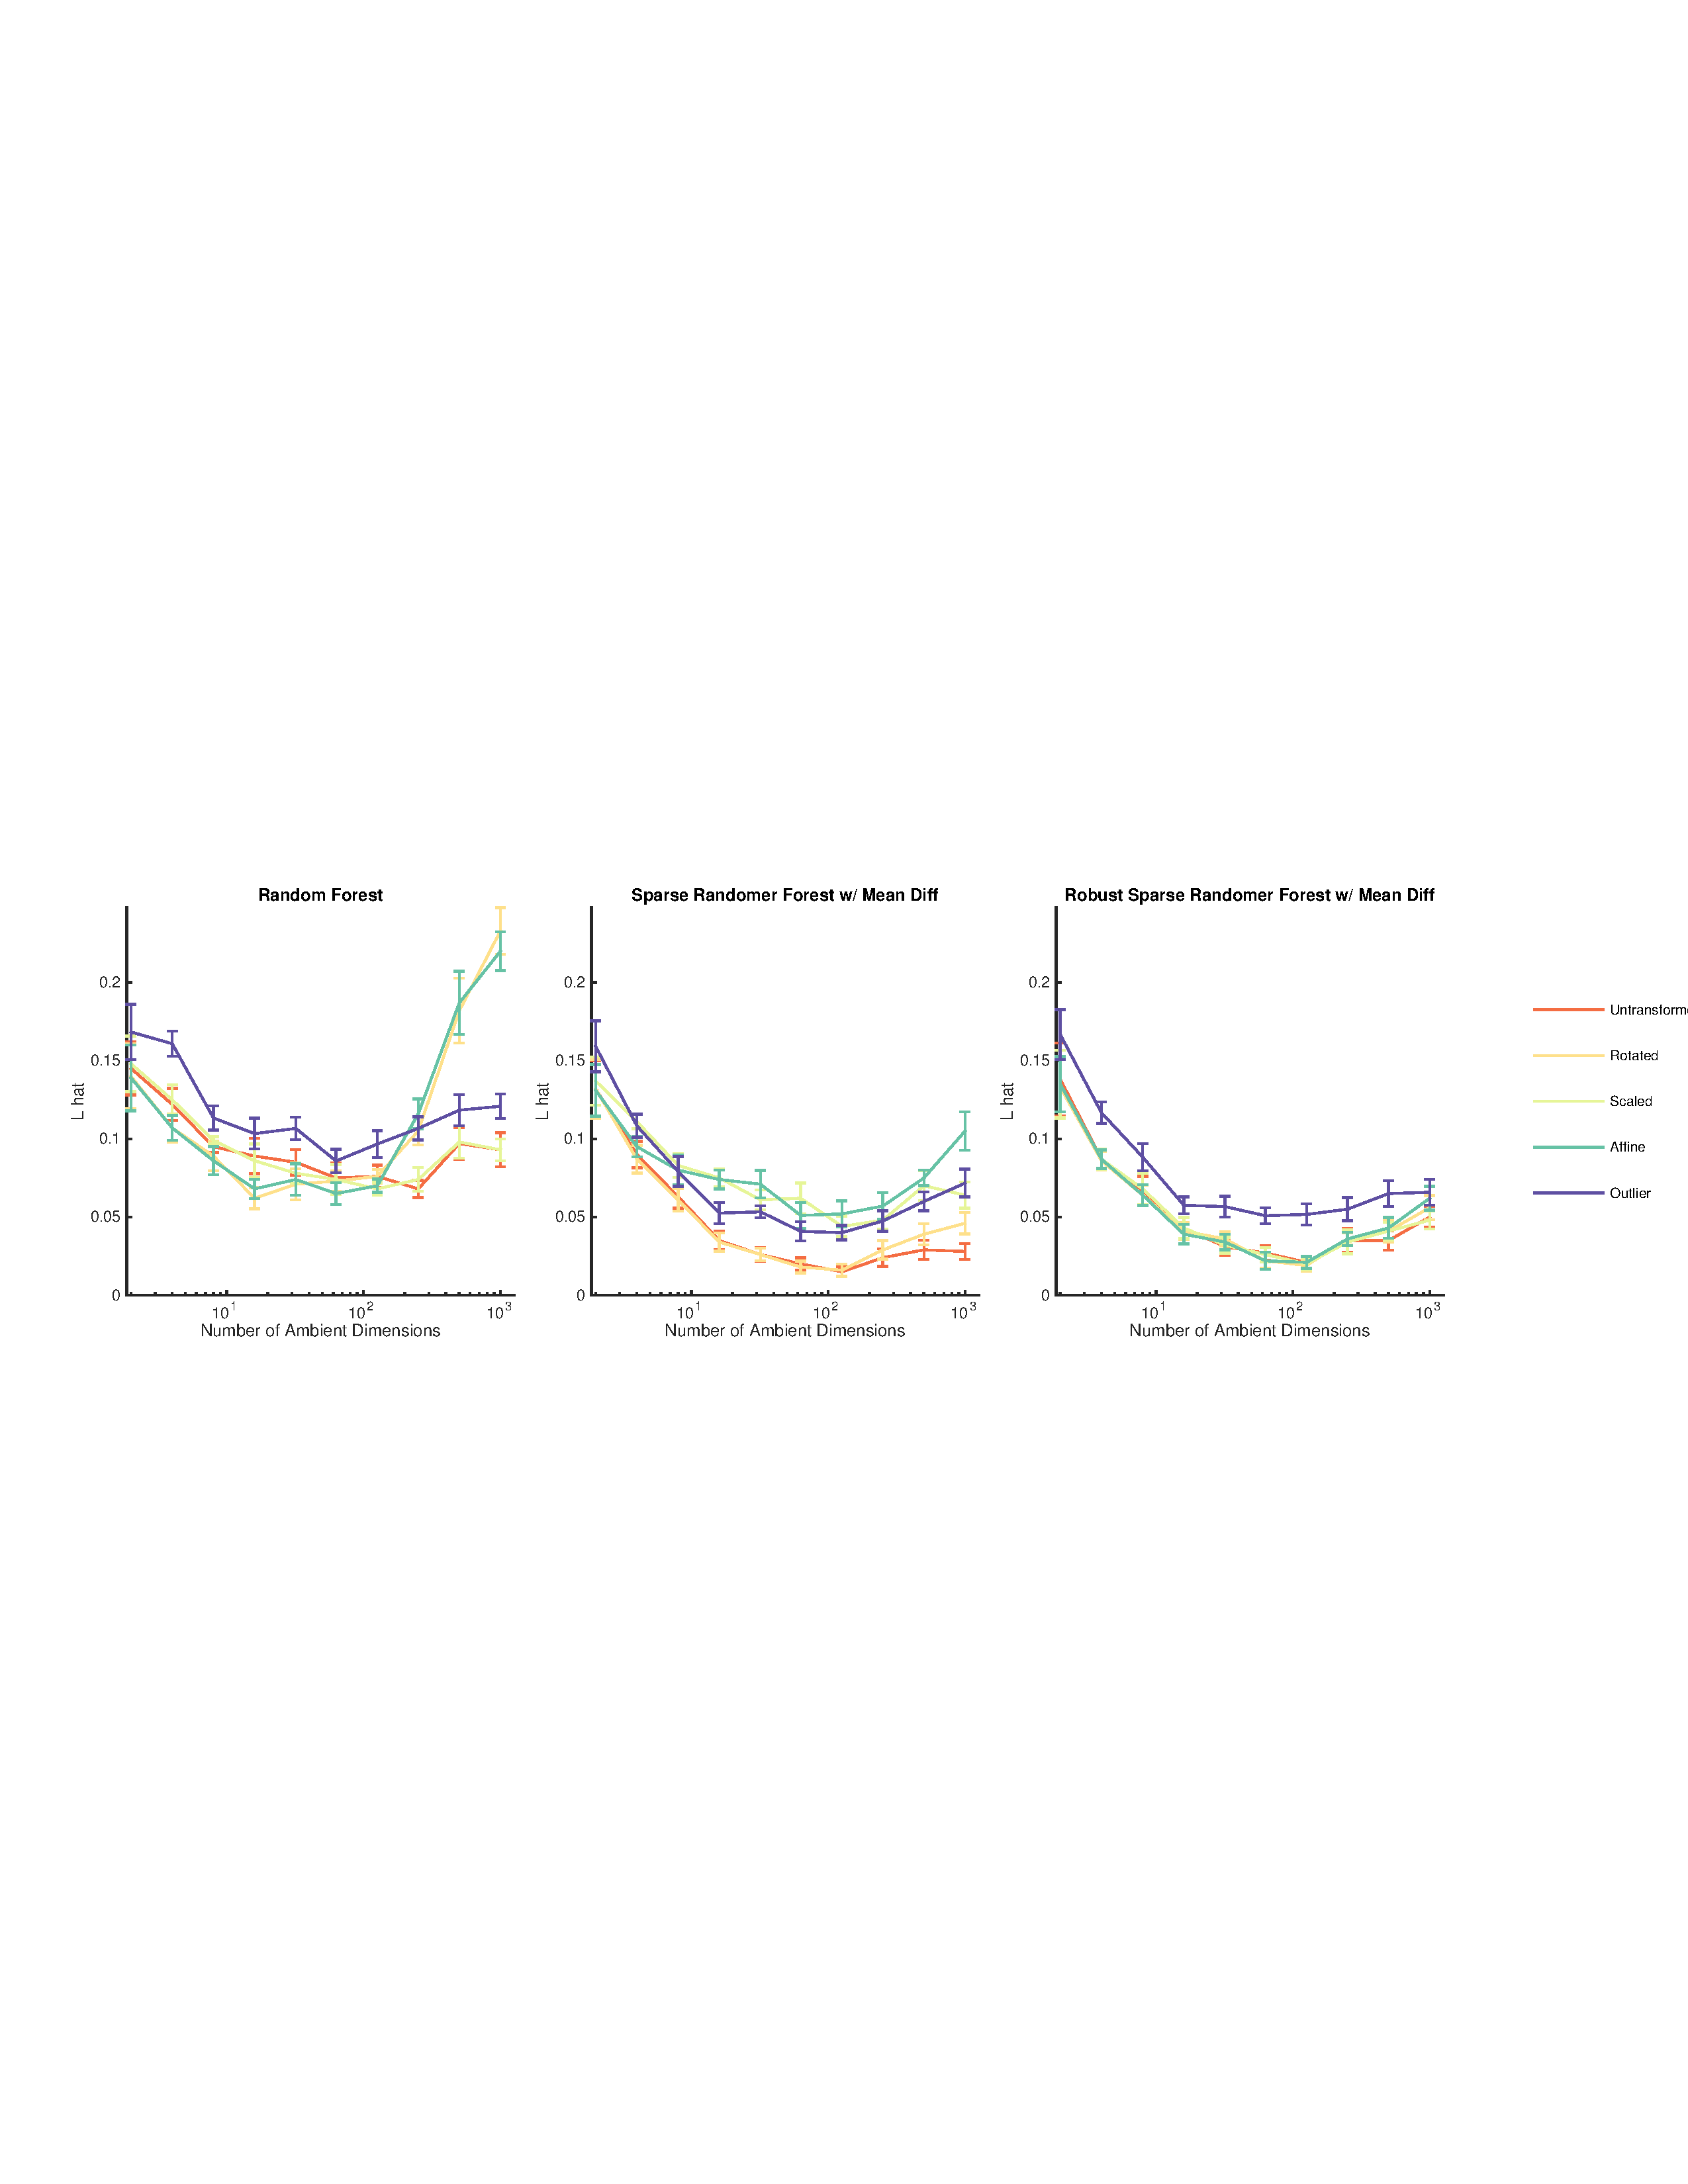
\includegraphics[trim=0in 0.9in 0in .09in, clip=true, width=\linewidth]{../Figures/pdf/Fig3_Invariance_v2}
\end{center}
\caption{The effect of various transformations applied to the Trunk (panels A-D) and Parity (panels E-H) simulations (see Methods for details) on classification performance of (A,E) RF, (B,F) RerF (s+d), (C,G) RerF (s+d+r), and (D,H) Fisherfaces. Specifically, we consider, rotations, scalings, and affine transformations, as well as introducing outliers. Classification performance of RF is compromised by rotations and therefore affine transformations as well. RerF(s+d) is invariant to rotation, but not scaling and therefore not affine transformation. RerF(s+d+r) is invariant to to affine transformations. Like RerF (s+d), Fisherfaces is invariant to rotation but not scaling. Note that all variants are reasonably robust to outliers.}
\label{fig:invar}
\end{figure}

\begin{figure}[h]
\begin{center}
%\framebox[4.0in]{$\;$}
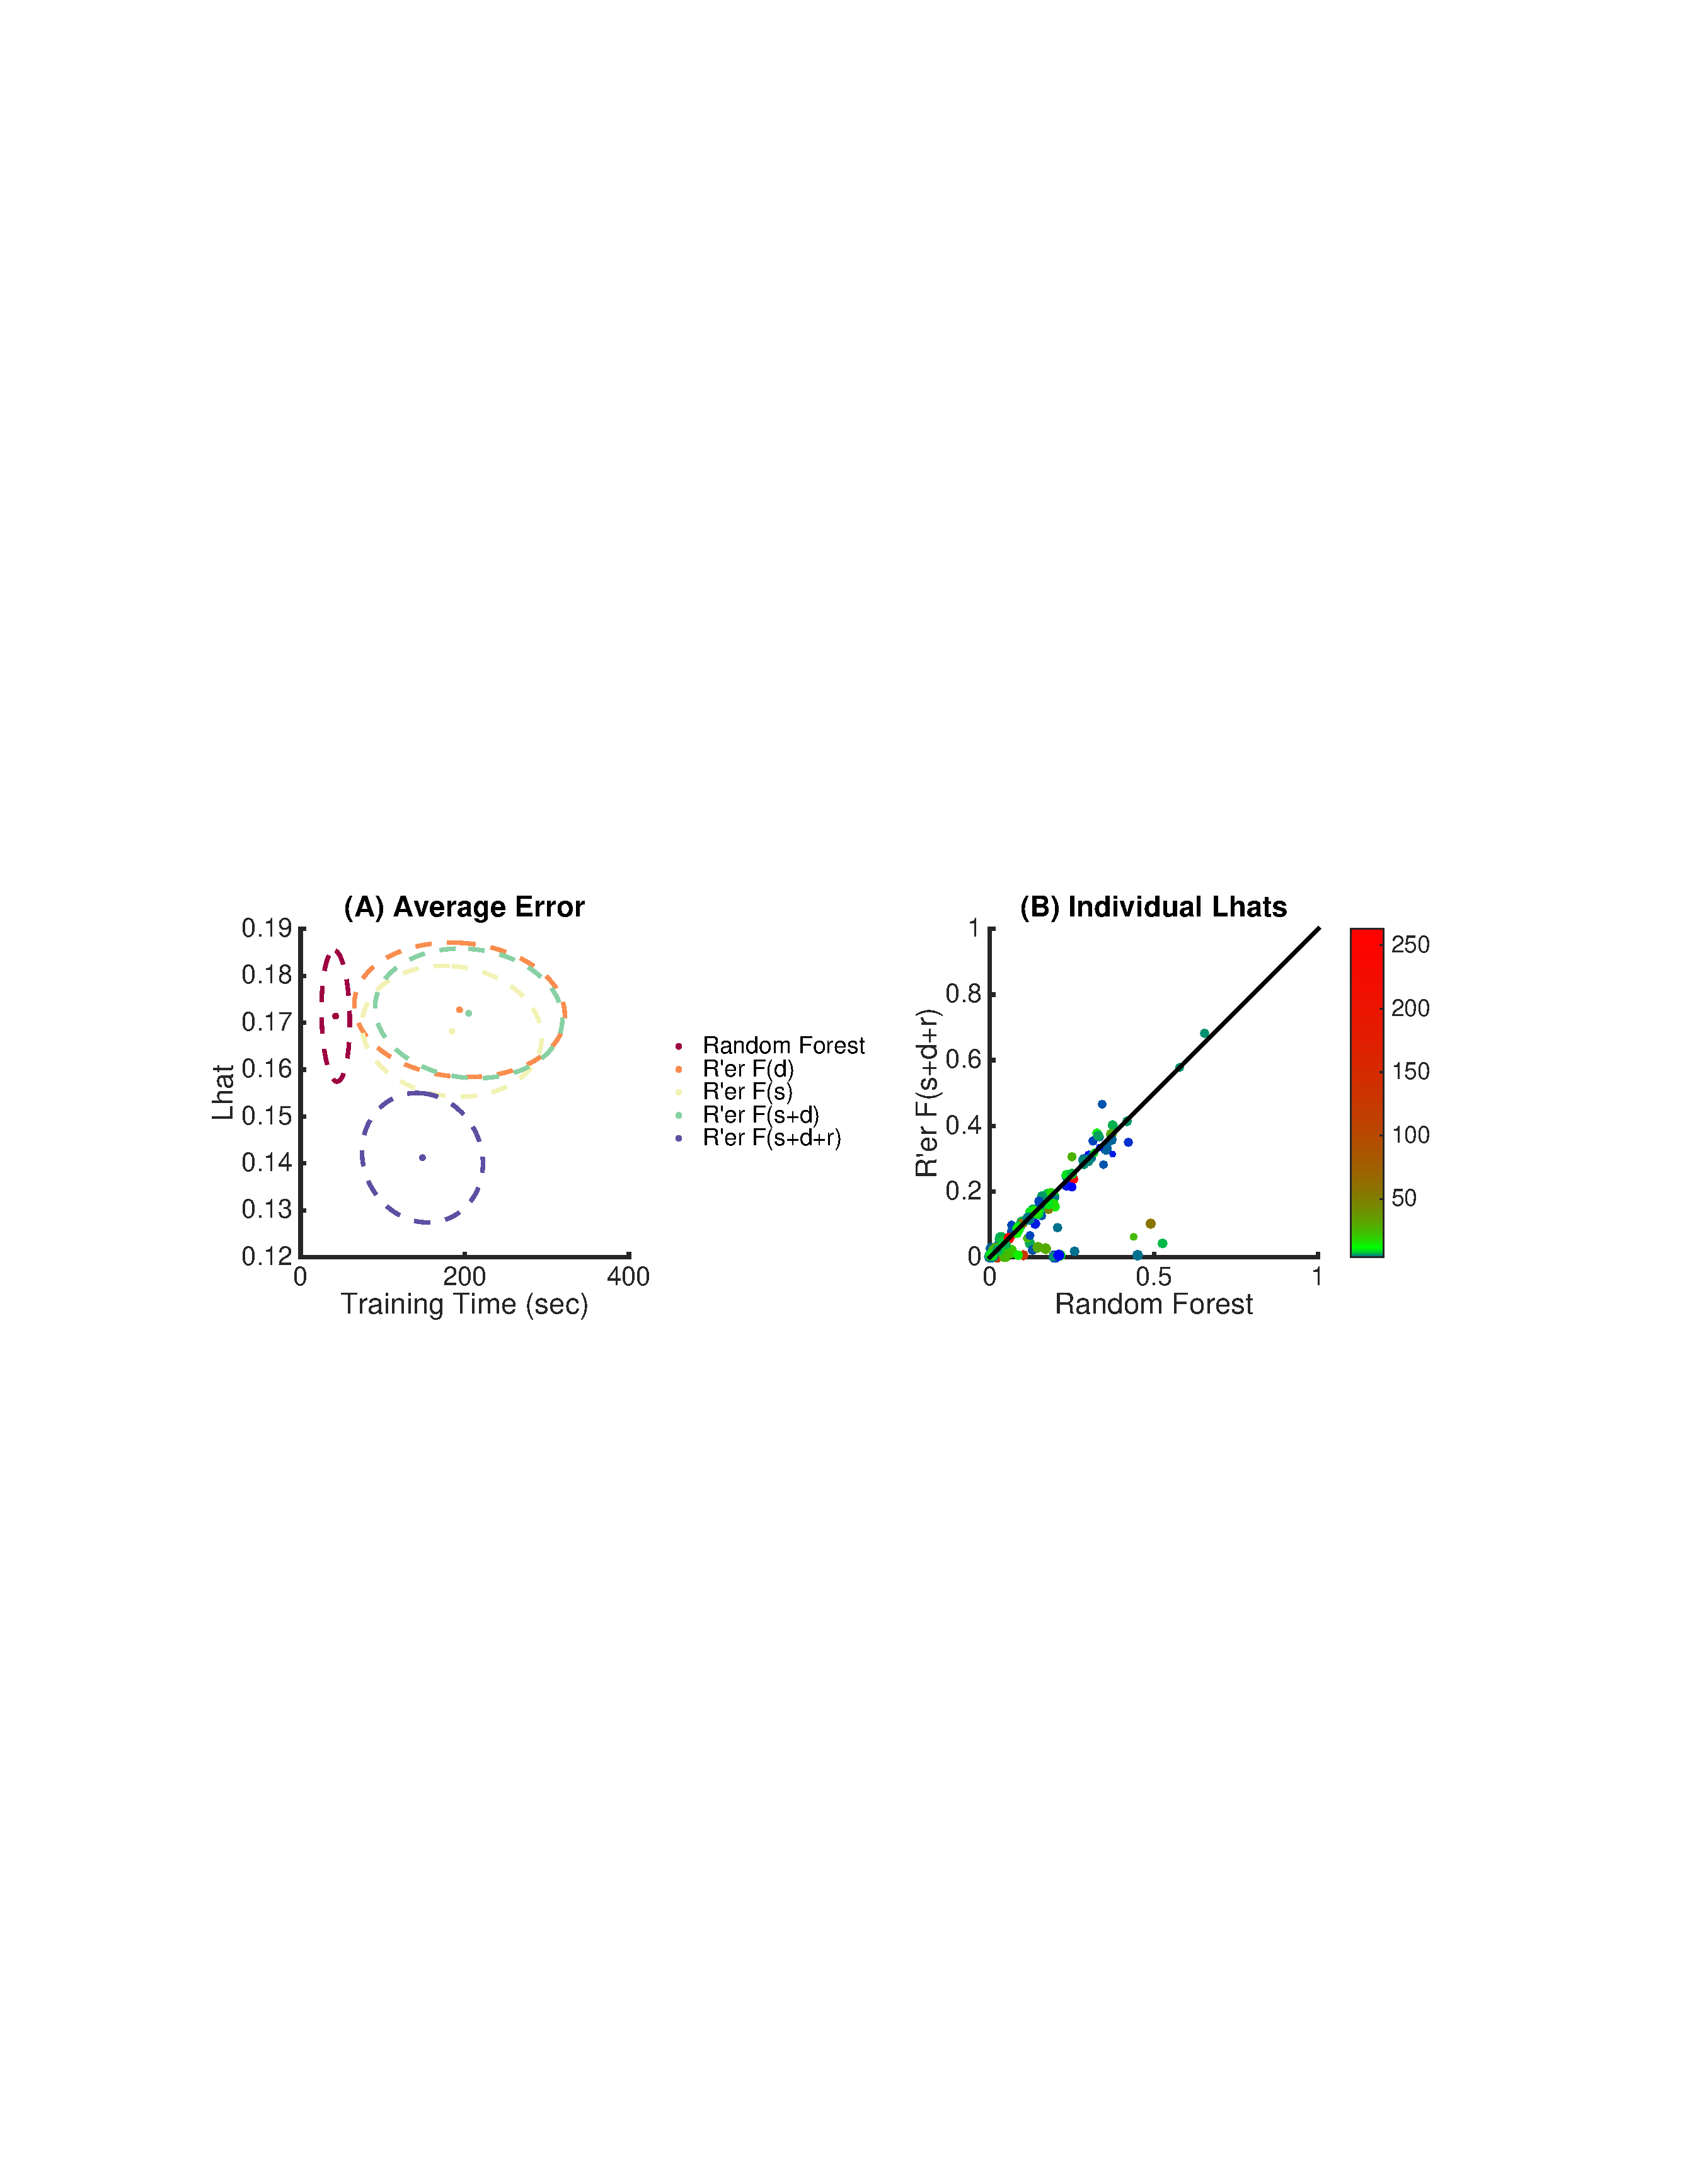
\includegraphics[trim=0in 2.3in 0in 2.3in, clip=true, width=\linewidth]{../Figures/pdf/Fig4}
\end{center}
\caption{(A) Classification error and training time of Random Forest and Randomer Forests variants for all 121 datasets from the benchmark comparison study by Caruana \cite{Caruana2008}. (A) Average (dots) and 0.1 standard deviation level sets (dashed lines) for each method. (B) Classification error of Randomer Forest (sparse+delta+robust) vs. that of Random Forest for each of the 121 datasets. The black line indicates equal classification error of the two algorithms. Color indicates dimensionality of the datasets and size of points indicates number of samples. Note that RerF almost always does as well, and often significantly better.}
\label{fig:benchmark}
\end{figure}
% Misclassification rates and training times were averaged over all 121 datasets (Fig 4).




\appendix
\setcounter{figure}{0}
\renewcommand\thefigure{A\arabic{figure}}

\begin{figure}[h]
\begin{center}
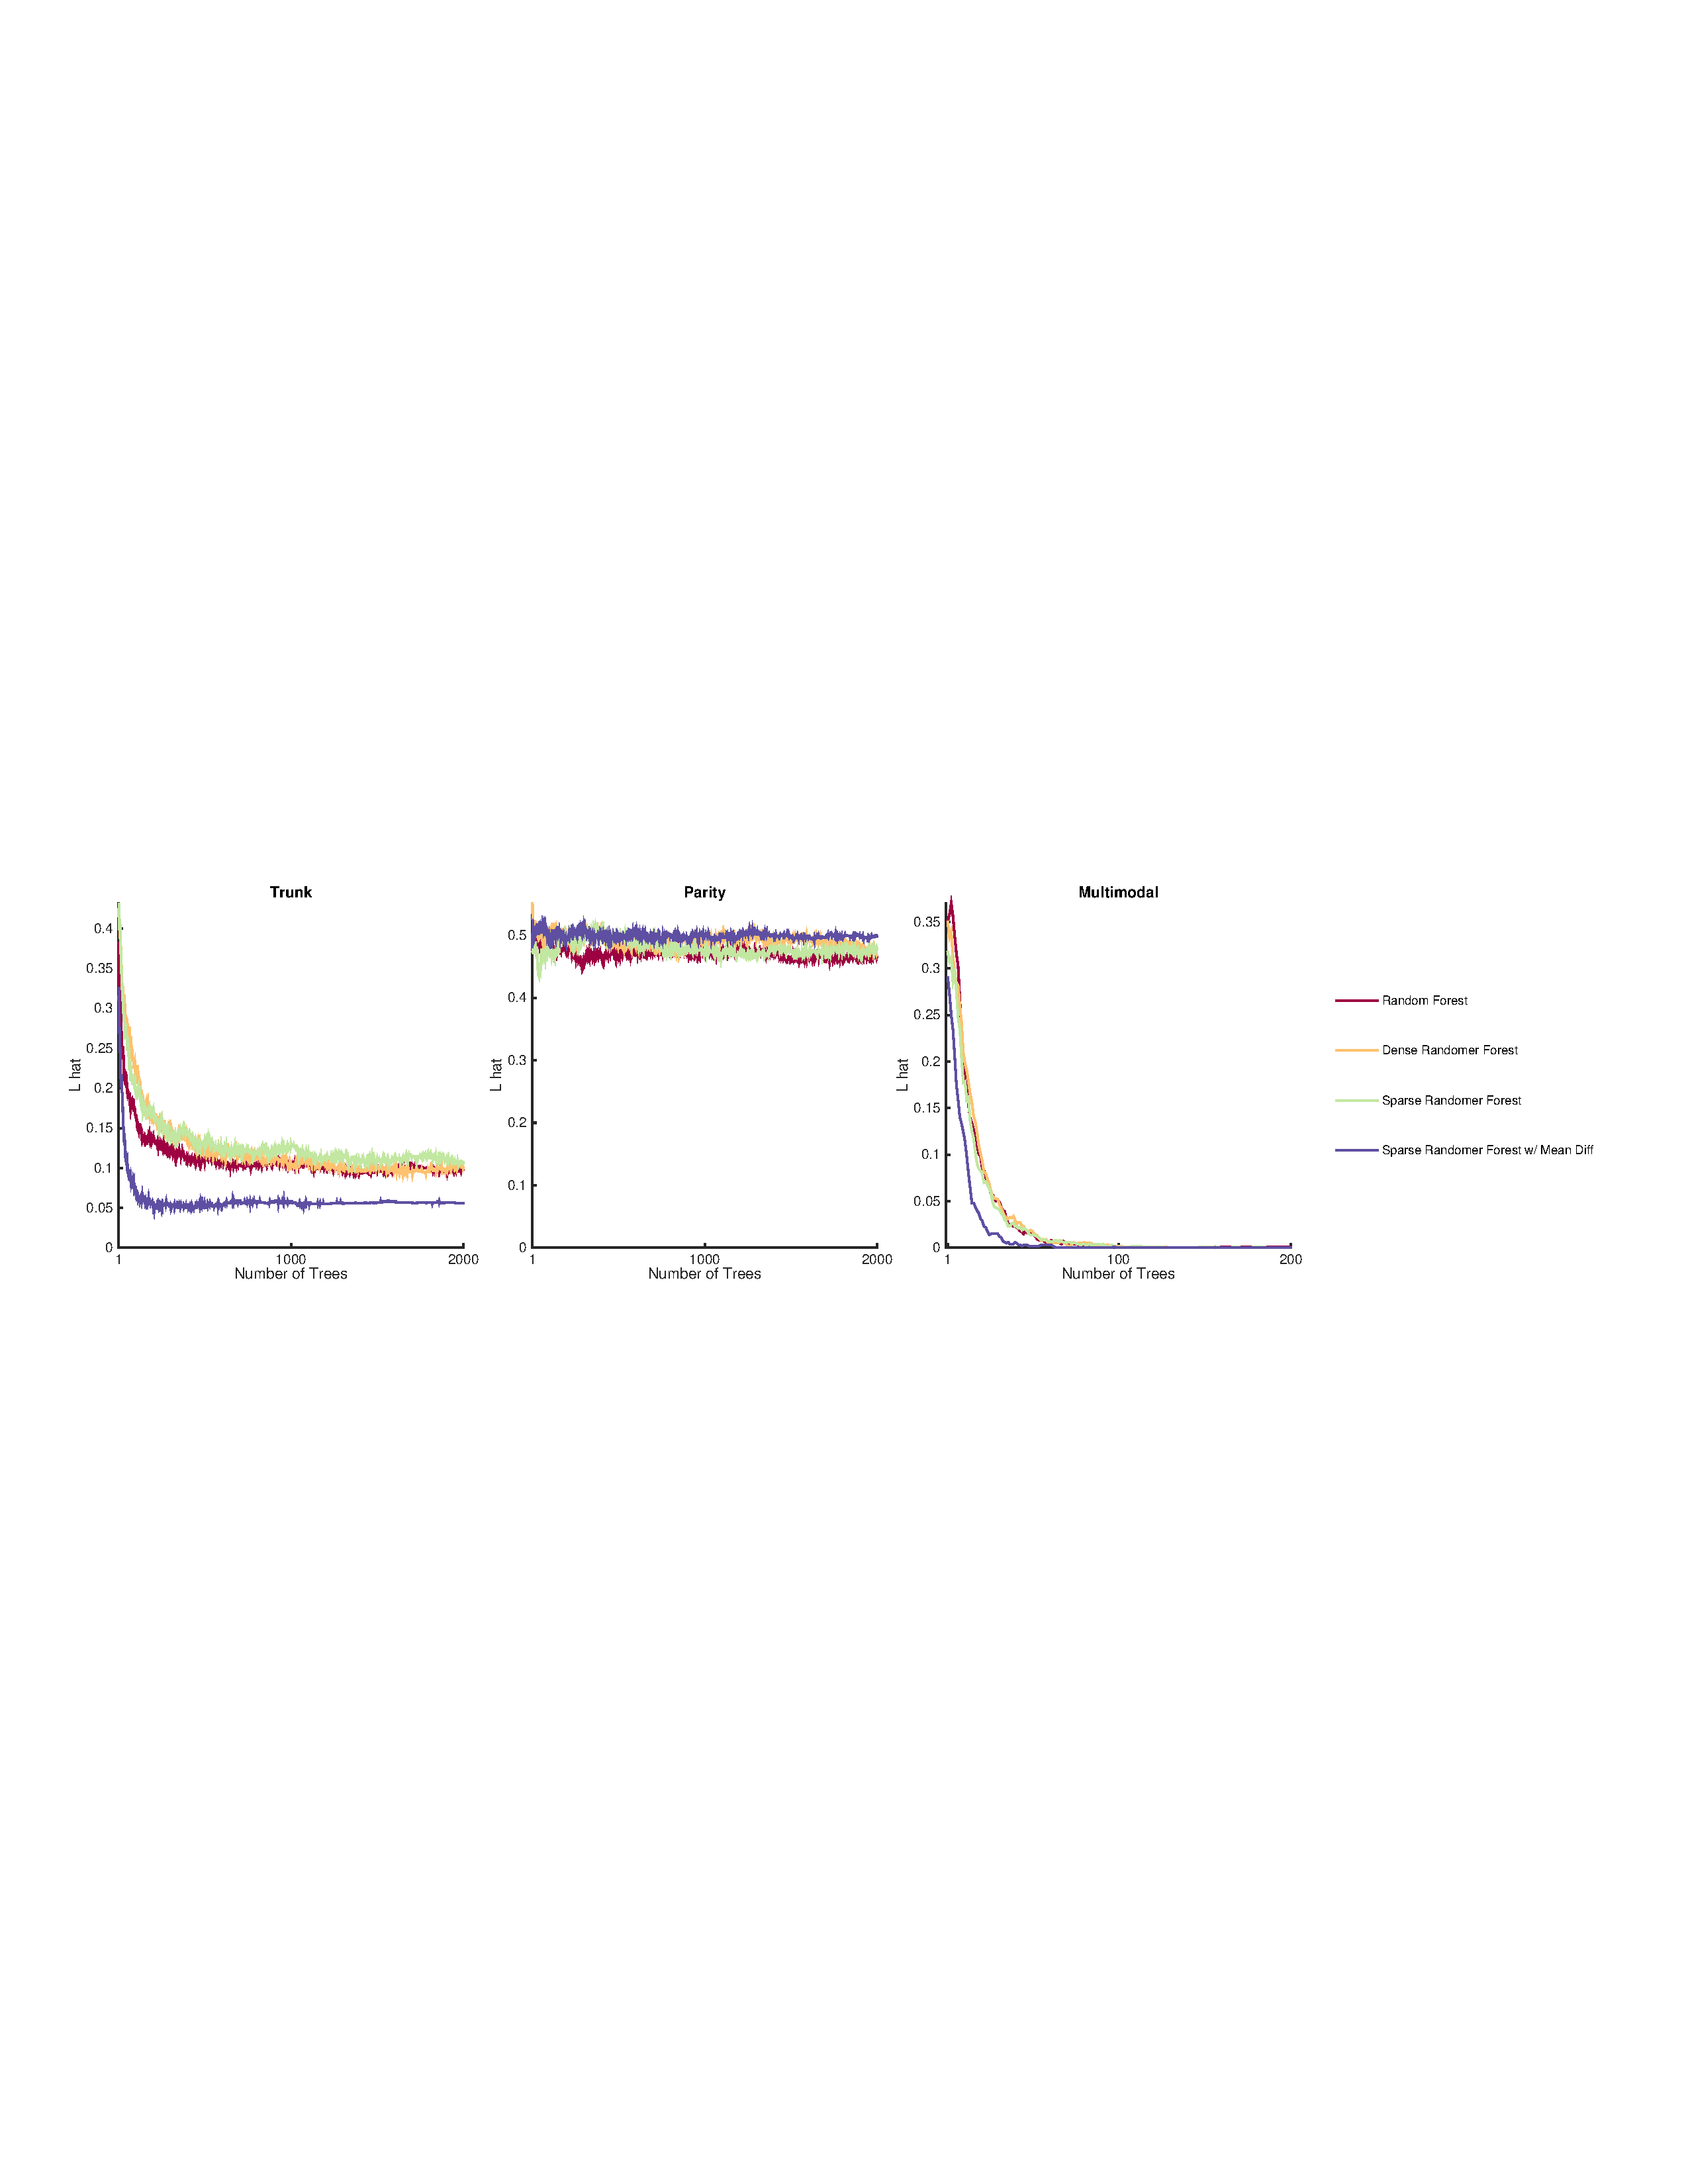
\includegraphics[trim=0in 8in 0in 8in, clip=true, width=\linewidth]{../Figures/pdf/Fig0_nTrees}
\end{center}
\caption{The number of trees until a stable misclassification rate is achieved for RF and the RerF variants in the Trunk, parity, and multimodal simulations. Simulation settings are the same as in Fig1. The number of ambient dimensions for panels A, B, and C were chosen to be 1000, 10, and 1000 respectively.}
\label{fig:ntrees}
\end{figure}

\begin{figure}[h]
\begin{center}
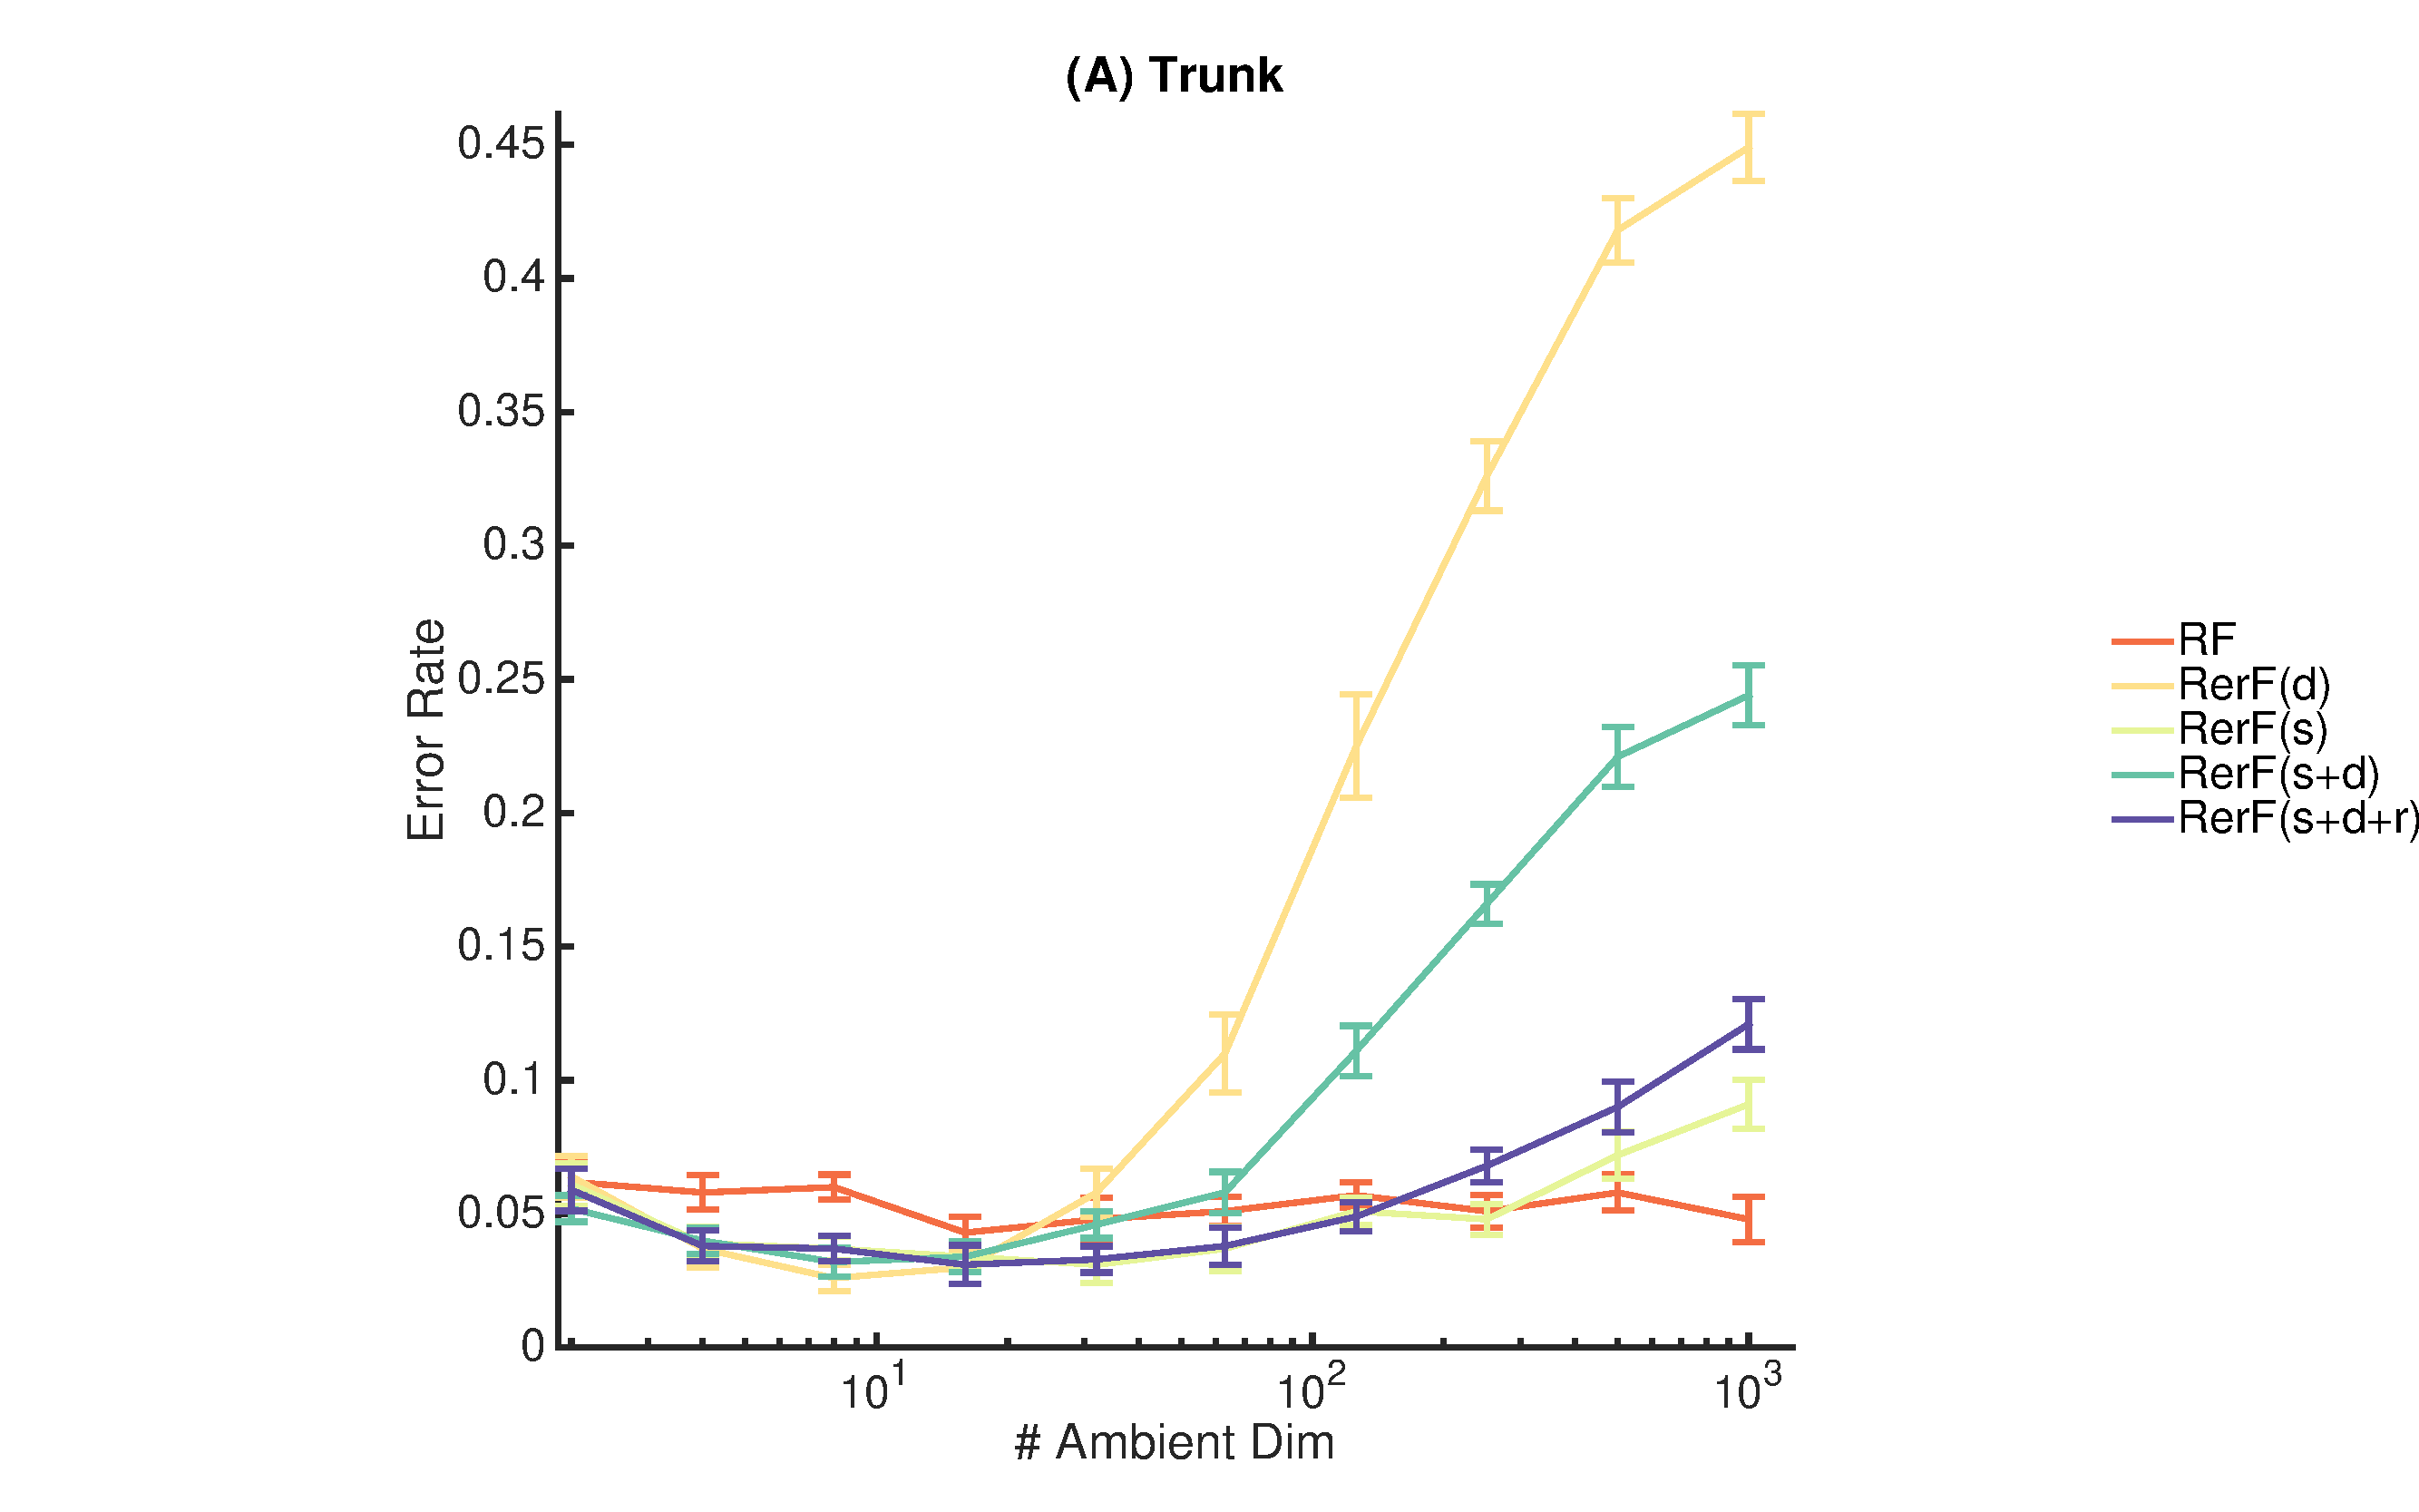
\includegraphics[trim=0in 0in 0in 0in, clip=true, width=\linewidth]{../Figures/pdf/Trunk_hard}
\end{center}
\caption{Classification performance comparing Random Forest (RF) to several variants of Randomer Forest (RerF) on the modified Trunk simulation setting. Here, the ith diagonal of the covariance matrices of both classes is equal to the inverse of the difference in means of the ith dimension between the two classes. For small values of p, all variants of RerF perform marginally better than RF. For large values of p, all variants of RerF perform worse than RF.}
\label{fig:trunk_hard}
\end{figure}

\bibliography{nips2015_tyler}
\bibliographystyle{IEEEtran}

\end{document}